\chapter{Estimation du seuil optimale par des indicateurs sonores}\label{annexe:optThreshold}

Dans la partie \ref{chap:grafic_nmf}, les seuils optimaux $t_{h,opt}$ par ambiance sonore ont été définis en considérant la NMF IS optimale avec $\beta$ = 2, $K$ = 300 et $w_t$ = 1 s. Ces seuils et les erreurs correspondantes  sont résumés dans le Tableau \ref{tab:erreur_optimiseAnn}.
et peuvent être considérés dans les réseaux de capteurs fixes où l'ESU peut être défini au préalable. Toutefois, leur prise en compte a un impact relativement faible sur les erreurs $MAE_g$. 

Cependant, une étude a été réalisée en vue de, non plus définir un seuil fixe selon l'ambiance sonore, mais de définir un seuil adaptatif basé sur des indicateurs physiques corrélés avec l'évolution des seuils optimaux. Cette adaptation permettrait de définir un seuil en fonction des ESU qui sont susceptibles en fonction de la période de l'année ou de la journée.

\begin{table}[h]
\centering
\caption{Erreurs $MAE_{60}$ minimales selon le seuil optimal $t_{h,opt}$ par ambiance sonore.}
\label{tab:erreur_optimiseAnn}
\resizebox{\textwidth}{!}{%
\begin{tabular}{L{4cm}C{2.5cm}C{2.5cm}C{2.5cm}C{2.5cm}C{2.5cm}}
\toprule
\textbf{ambiance} & \textbf{Parc} & \textbf{Rue Calme} & \textbf{Rue Bruyante} & \textbf{Rue très bruyante} & $\mathbf{MAE_{60}}$ \\
\midrule
seuil fixe $t_h$ & 0,35 & 0,35 & 0,35 & 0,35 & 0,35 \\
erreur $MAE_{60}$ & 2,13 ($\pm$ 3,84) & 1,62 ($\pm$ 1,85) & 0,57 ($\pm$ 0,54) &  0,32 ($\pm$ 0,20) & 1,16 ($\pm$ 0,86) \\
\midrule
seuil optimal $t_{h,opt.}$ & 0,38 & 0,35 & 0,33 & 0,31 & - \\
erreur $MAE_{60}$ & 2,03 ($\pm$ 3,47) & 1,62 ($\pm$ 1,85) & 0,56 ($\pm$ 0,67) & 0,28 ($\pm$ 0,31) & 1,12 ($\pm$ 0,83)\\
\bottomrule
\end{tabular}}
\end{table}


Des outils de classification pour les environnements sonores existent déjà dans la littérature et sont basés sur des indicateurs simples (\cite{can_describing_2015}, \cite{rychtarikova2013soundscape}) ou sur des outils plus complexes comme dans \cite{salamon2015unsupervised}.
Dans le cadre de ces travaux, il est nécessaire que ces indicateurs soient simples en vue de les considérer sur l'ensemble des types de mesures possibles (fixes, mobiles, participatives) et dont les puissances de calculs sont limités. Ainsi, nous considérons une approche simple basée sur l'estimation d'indicateurs de niveaux sonores.
Plusieurs indicateurs sont considérés comme des niveaux sonores par bandes de tiers d'octaves ($L_{500}$, $L_{1000}$, $L_{2000}$, $L_{5000}$) ainsi que des niveaux sonores fractiles ($L_{10}$, $L_{50}$, $L_{90}$). Ces derniers expriment les niveaux sonores dépassés pendant une période définie. Ainsi $L_{10}$ exprime le niveau sonore dépassé 10 $\%$ du temps, cela résume les hauts niveaux sonores, à l'inverse l'indice $L_{90}$ traduit le niveau sonore dépassé 90 $\%$ du temps et exprime donc l'équivalent du bruit de fond sonore d'une scène.

Toutefois, cette approche se heurte à la calibration des scènes sonores. En effet, les enregistrements qui ont servi à la construction du corpus \textit{SOUR} n'ont pas été accompagnés d'un fichier de calibration. Il n'a donc pas été possible d'estimer leur niveau sonore exacte et donc impossible de calibrer les scènes sonores du corpus. Leur niveaux sonores absolus ne sont donc pas être estimés. Une approximation avait été réalisée dans le Tableau \ref{tab:obsScene} à partir des informations données dans la Figure \ref{fig:parcoursGRAFIC}, dans le but d'harmoniser les fichiers audio par ambiances et mais celle-ci n'est pas suffisante ici.

En revanche, en considérant que les scènes du corpus \textit{SOUR} sont représentatives d'enregistrements sonores urbains, si les niveaux absolus des indicateurs de niveaux sonores ne sont pas estimés par défaut de calibration, leurs rapports entre eux l'est tout de même. En effet, quelque soit le niveau sonore global de la scène, si la distribution des évènements sonores et leur répartition dans la scène est correcte, l'estimation de niveaux sonores relatifs, quelque soit le niveau sonore global, restent correcte.
Ainsi les différences entre les niveaux par bandes de tiers d'octaves et entre les niveaux fractiles peuvent être considérés : 

\begin{subequations}\label{eq:delta_L}
\begin{align}
\Delta_{L_{500}-L_{1000}} &= L_{500}-L_{1000}, \\
\Delta_{L_{500}-L_{2000}} &= L_{500}-L_{2000}, \\
\Delta_{L_{500}-L_{5000}} &= L_{500}-L_{5000}, \\
\Delta_{L_{1000}-L_{2000}} &= L_{1000}-L_{2000}, \\
\Delta_{L_{1000}-L_{5000}} &= L_{1000}-L_{5000}, \\
\Delta_{L_{2000}-L_{5000}} &= L_{500}-L_{5000}, \\
\Delta_{L_{10}-L_{50}} &= L_{10}-L_{50}, \\
\Delta_{L_{10}-L_{90}} &= L_{10}-L_{90}, \\
\Delta_{L_{50}-L_{90}} &= L_{50}-L_{90}.
\end{align}
\end{subequations}

\begin{figure}[h]
\centering
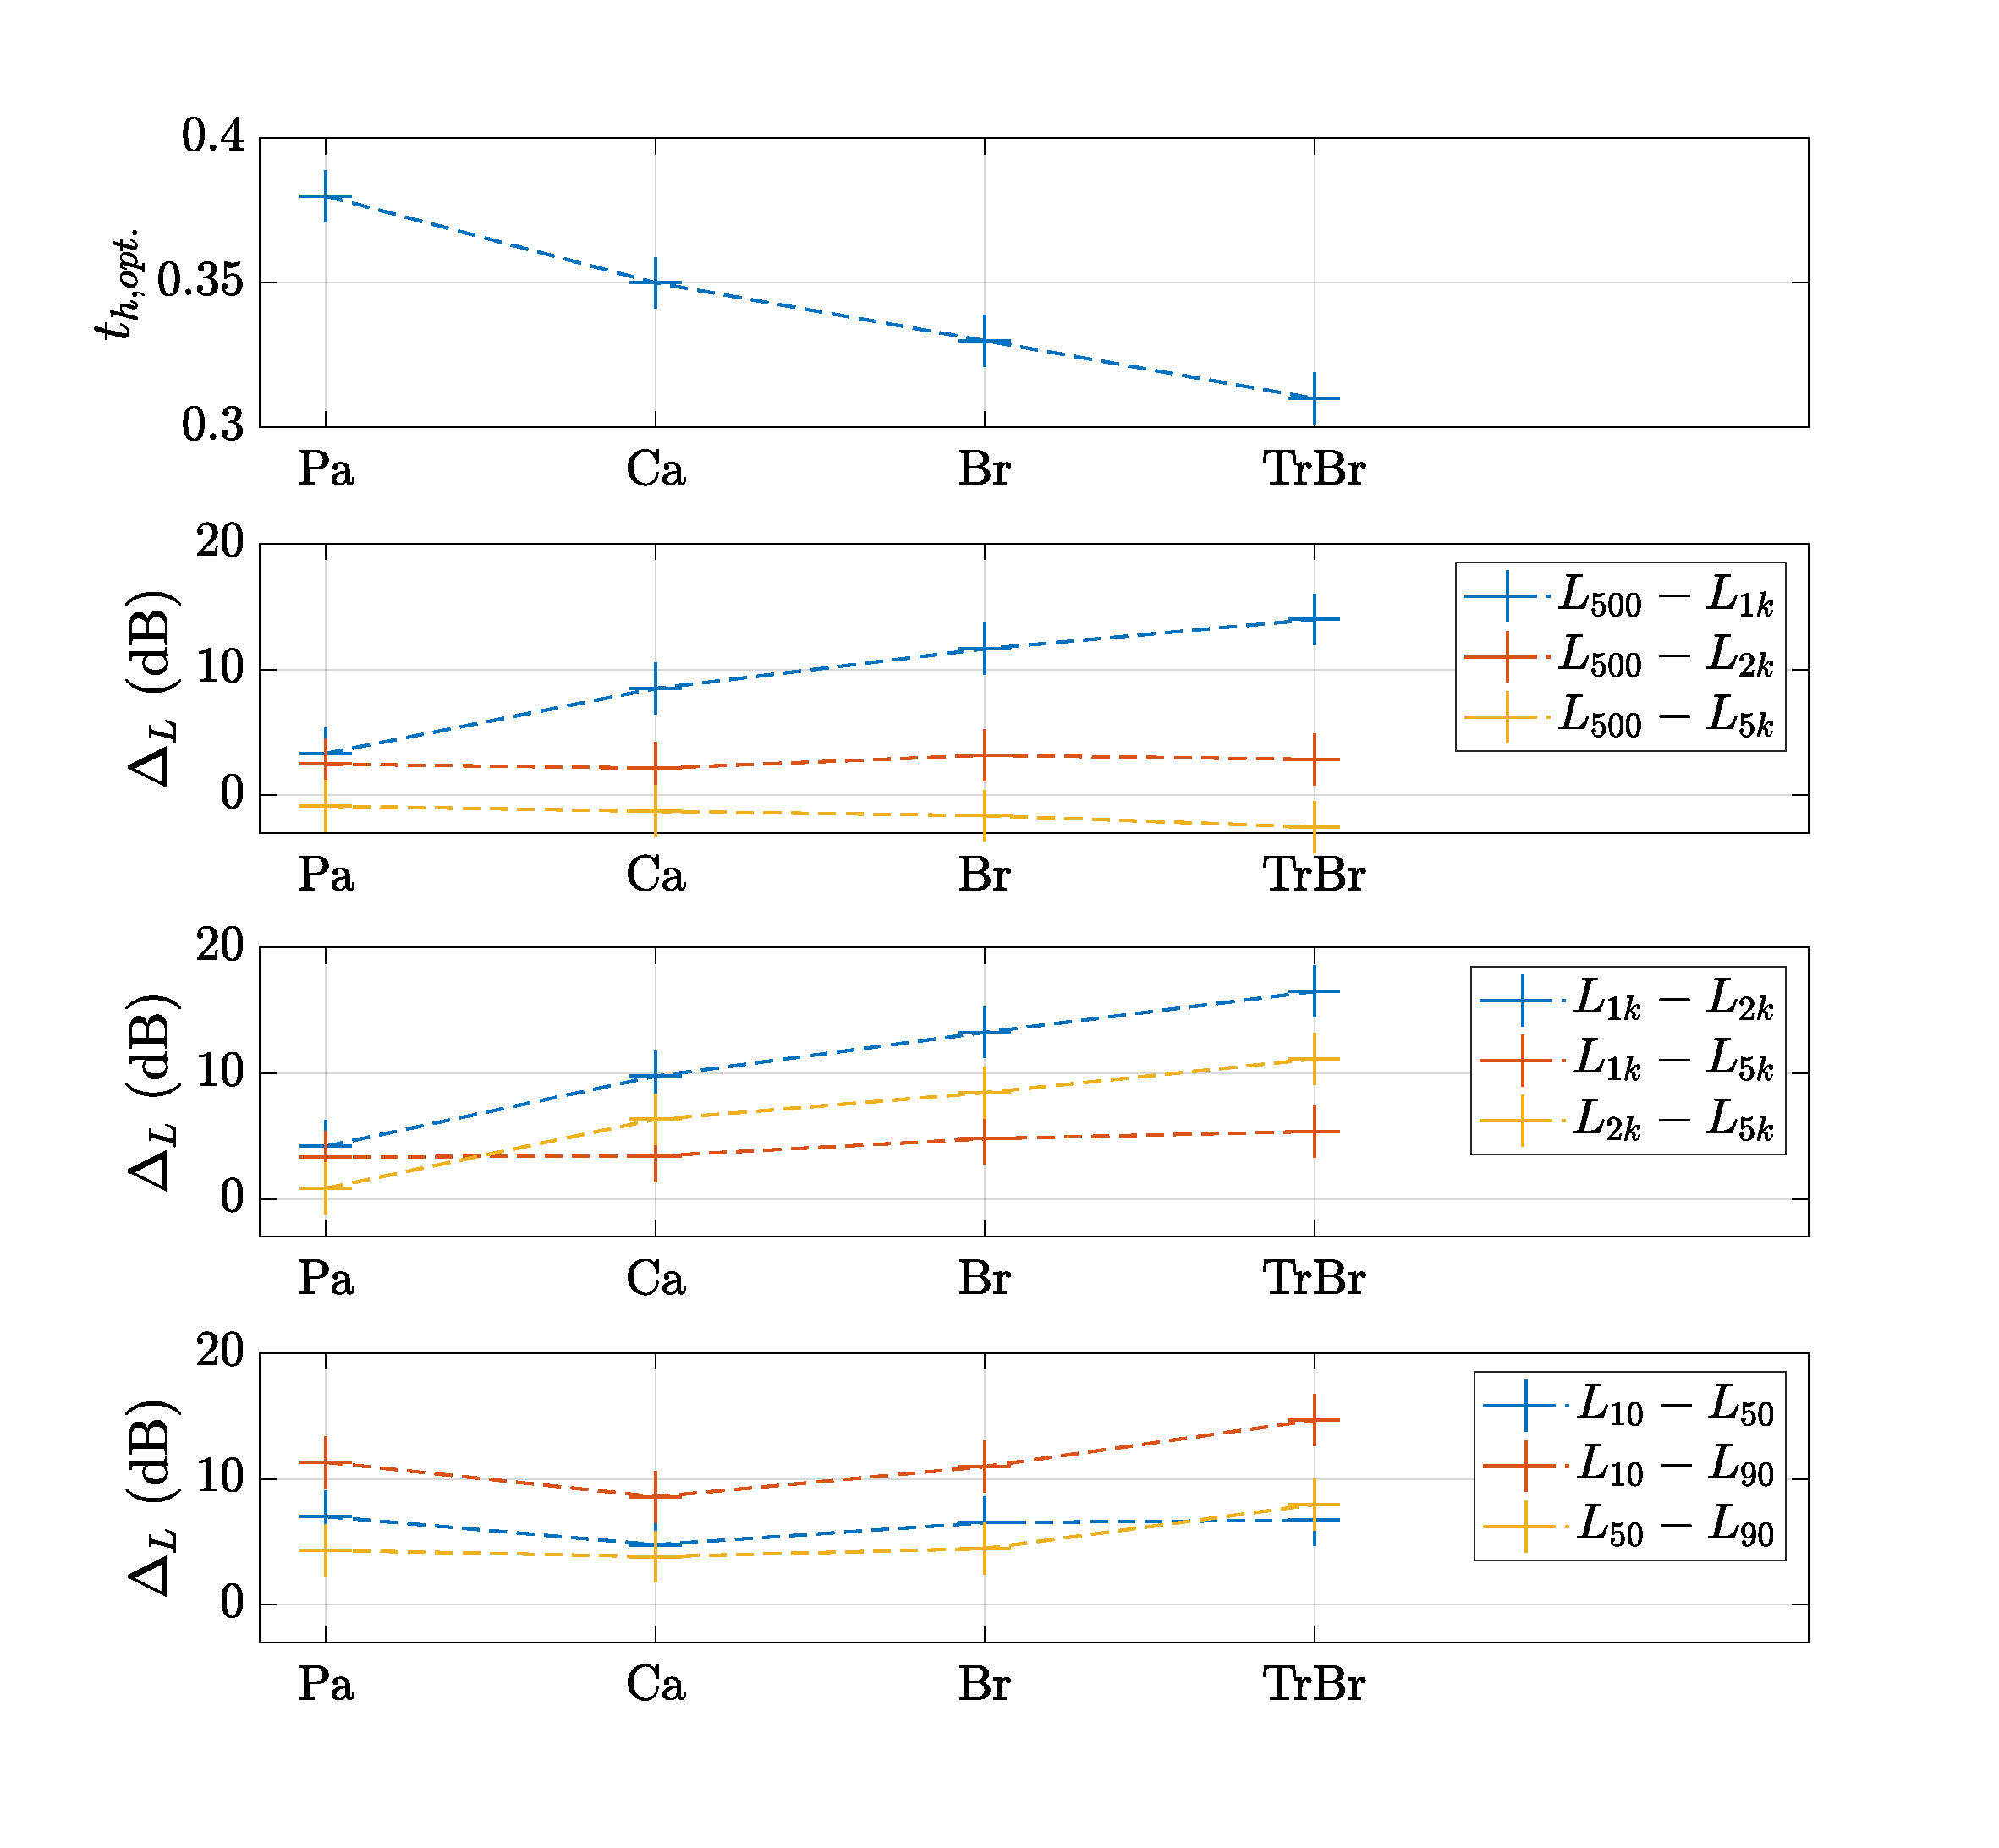
\includegraphics[width=0.9\linewidth]{./figures/resultats/deltaL_opt.pdf}
\caption{Évolution des seuils optimaux et des indicateurs $\Delta_L$ selon les ambiances.}
\label{fig:delta_L}
\end{figure}


La Figure \ref{fig:delta_L} résume les évolutions du seuil optimal et des indicateurs $\Delta_{L_x-L_y}$ par ambiance sonore. \`A partir de ces valeurs, les corrélations entre l'évolution du seuil optimale par ambiance sonore et celles des indicateurs sont alors calculées pour déterminer celui qui évolue de la même manière que $t_{h,opt}$. Les valeurs absolues des corrélations sont résumées dans le Tableau \ref{fig:correlation}.

\begin{figure}[h]
\centering
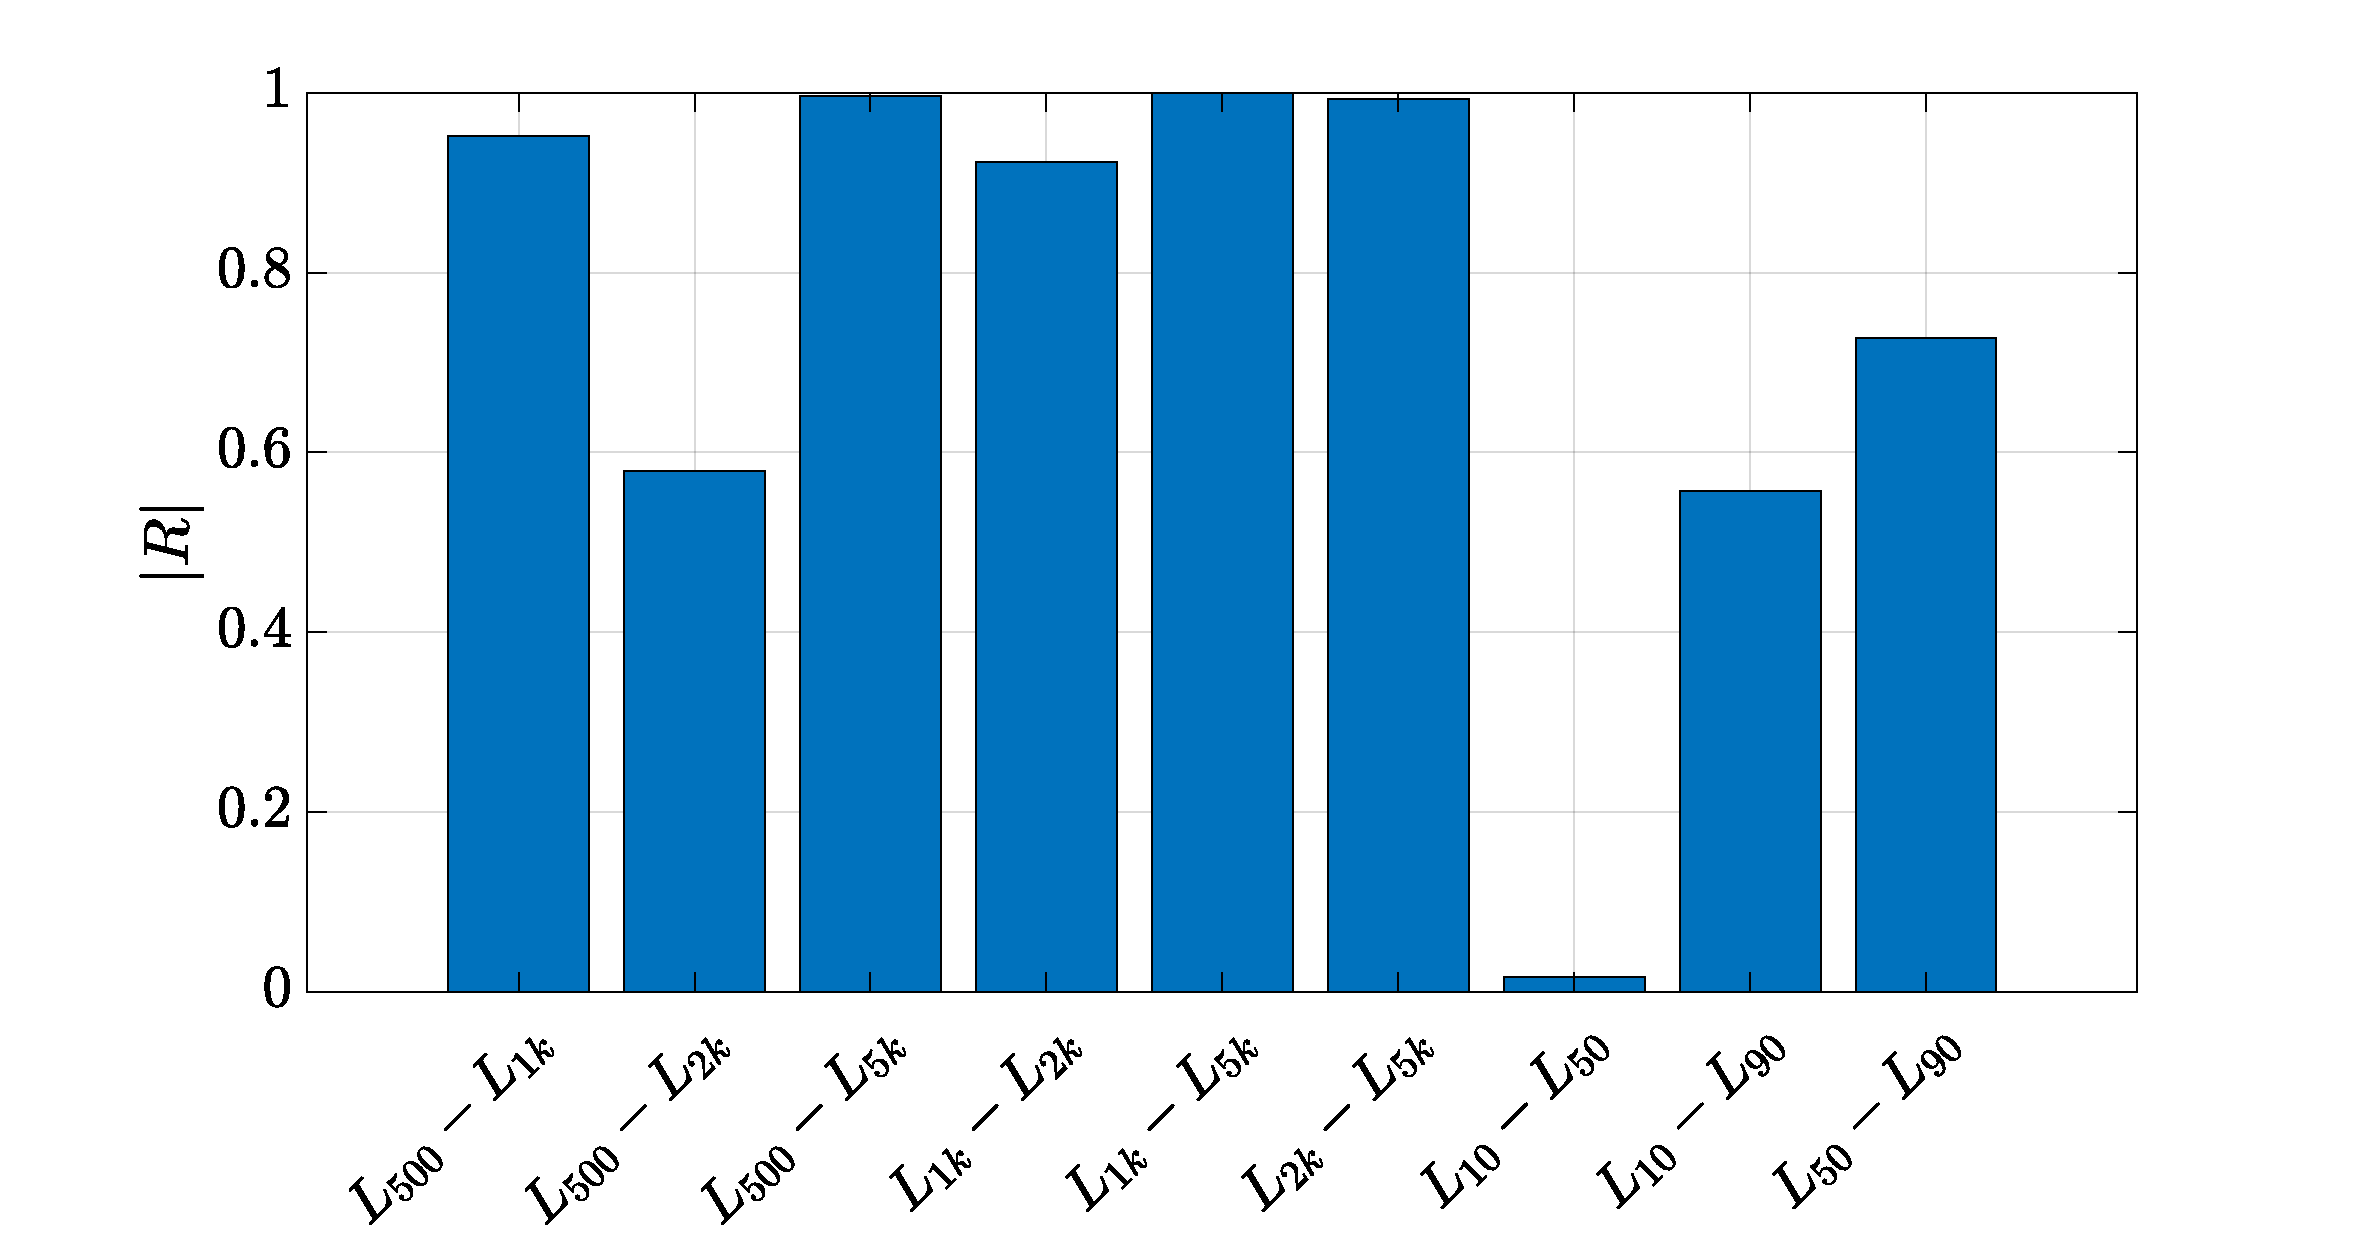
\includegraphics[width=0.9\linewidth]{./figures/resultats/Opt_correlation.pdf}
\caption{Corrélations entre l'évolution des seuils optimaux et des indicateurs $\Delta_{L_x-L_y}$.}
\label{fig:correlation}
\end{figure}

On obtient une forte corrélation pour les indicateurs $\Delta_{L_{1k}-L_{5k}}$, $\Delta_{L_{500}-L_{5k}}$ et $\Delta_{L_{2k}-L_{5k}}$. Avec une différence entre un niveau situé dans les basses (500 Hz) ou moyennes fréquences (1 kHz et 2 kHz) basses avec une niveau situé dans les plus hautes fréquences (5 kHz), on réussit à définir aux mieux les environnements sonores. En effet, les ambiances \textit{Parc} et \textit{Rue calme} avec la présence d'oiseaux sont susceptibles de contenir plus de hautes fréquences alors que la source \textit{trafic} est moins présente. À l'inverse, pour \textit{Rue bruyante} et \textit{Rue très bruyante} possèdent une plus grande proportion de basses fréquences. 
Les indicateurs basés sur la différence des niveaux fractiles et celui basé sur la différence entre le niveaux sonores des bandes de 500 Hz et de 2 kHz sont ceux obtenant les plus faibles corrélations. Là où les autres indicateurs suivent une évolution quasi linéaire, comme celle des seuils optimaux, ces 4 indicateurs ont des valeurs plus faibles pour l'ambiance \textit{calme}, ce qui diminue leur corrélation.

\begin{figure}[h]
\centering
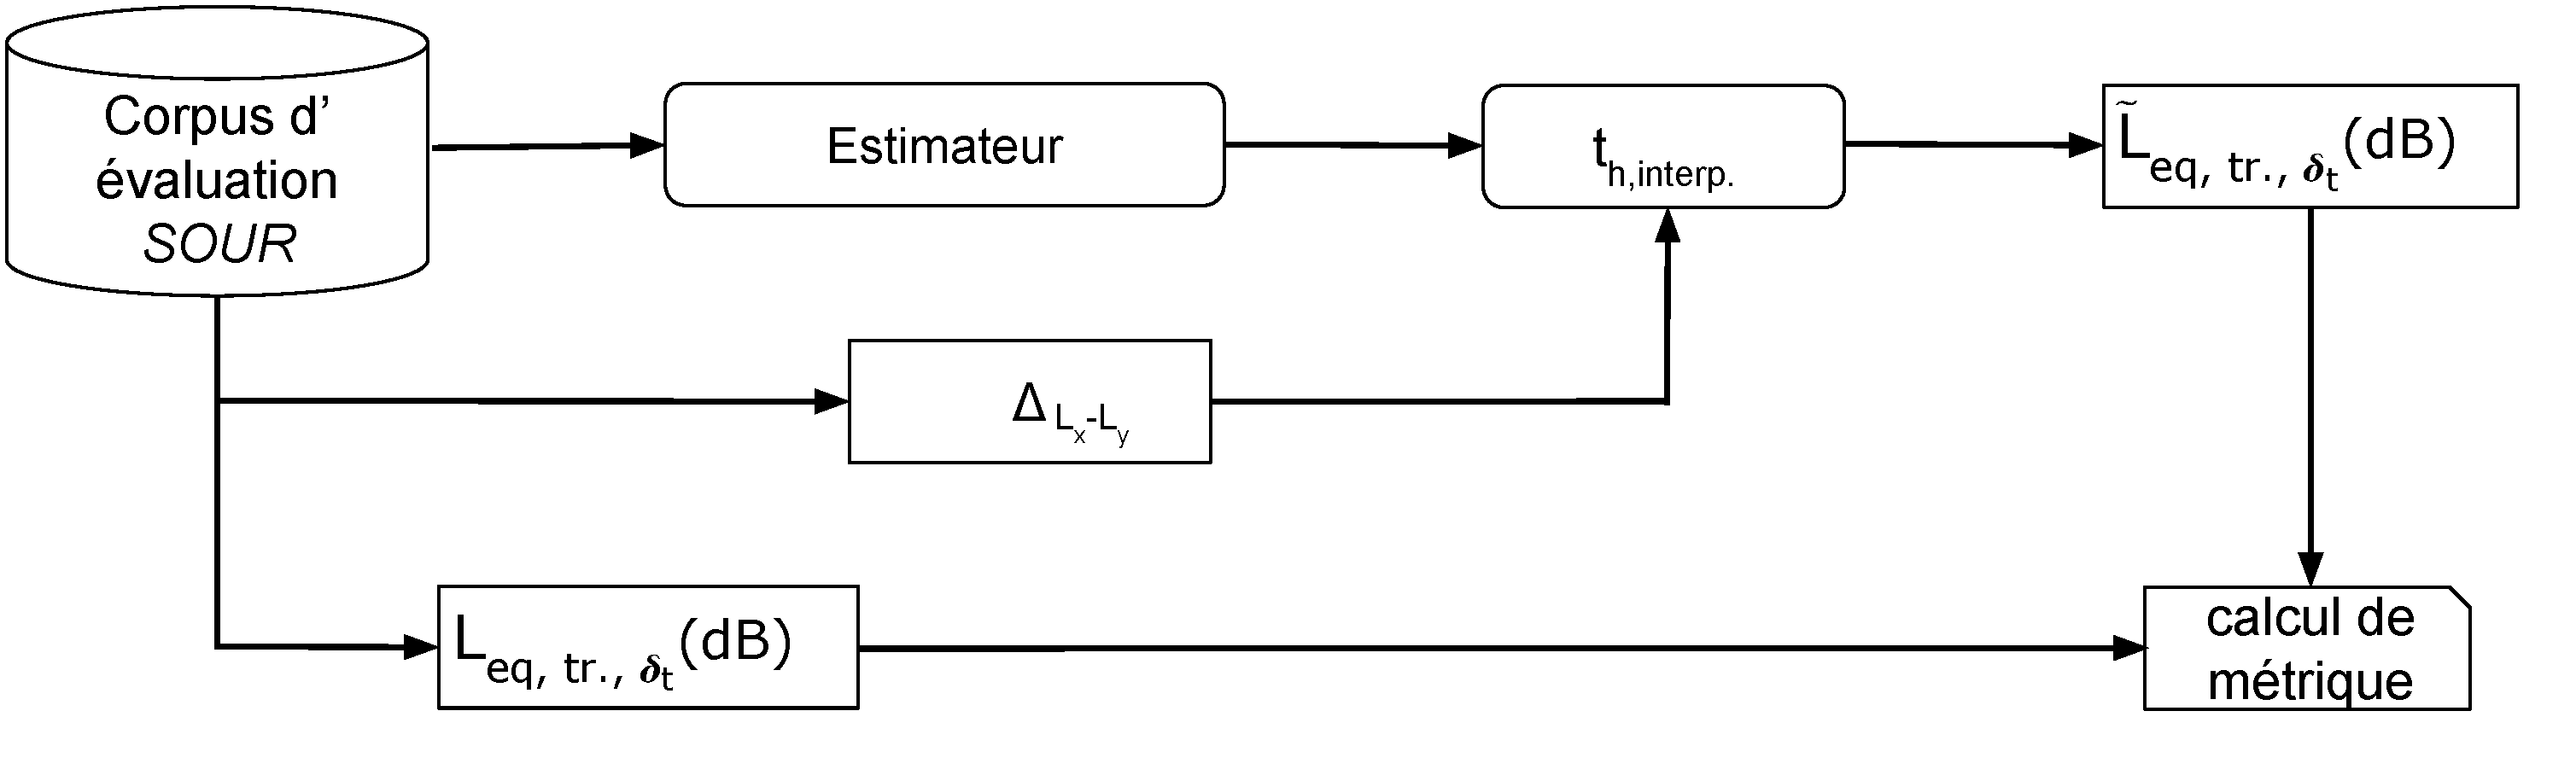
\includegraphics[width=.9\linewidth]{./figures/NMF/bloc_diagram_interpolation.pdf}
\caption{Schéma de principe de la détermination du niveau sonore du trafic par seuil interpolé.}
\label{fig:schema_NMFIS_interp}
\end{figure}

De ces indicateurs et des ces seuils optimaux, la NMF IS ($\beta$ = 2, $K$= 300, $w_t$ = 1 s) est de nouveaux appliquée sur le corpus \textit{SOUR} où la valeur du seuil $t_h$ n'est plus définie au préalable mais à partir de l'estimation d'un des indicateurs : pour chaque scène, un indicateur $\Delta_{L_x-L_y}$ est calculé, puis, la valeur seuil $t_{h,interp.}$ est trouvée par interpolation (voir Figure \ref{fig:interpolation}). Le principe de la méthode est présente par un schéma en Figure \ref{fig:schema_NMFIS_interp}.
Toutefois, si l'indicateur $\Delta_{L_x-L_y}$ de la scène excède les valeurs limites déterminés aux ambiances \textit{parc} et \textit{rue très bruyante}, les seuils prendront les valeurs optimales $t_{h,opt.}$ de ces ambiances afin de ne pas réaliser d'extrapolation.  À partir de l'évolution de l'indicateur en fonction des valeurs seuil, on réalise une simple interpolation pour déterminer un seuil $t_h$ plus précis qui s'adapte ainsi à chaque scène sonore.


\begin{figure}[h]
\centering
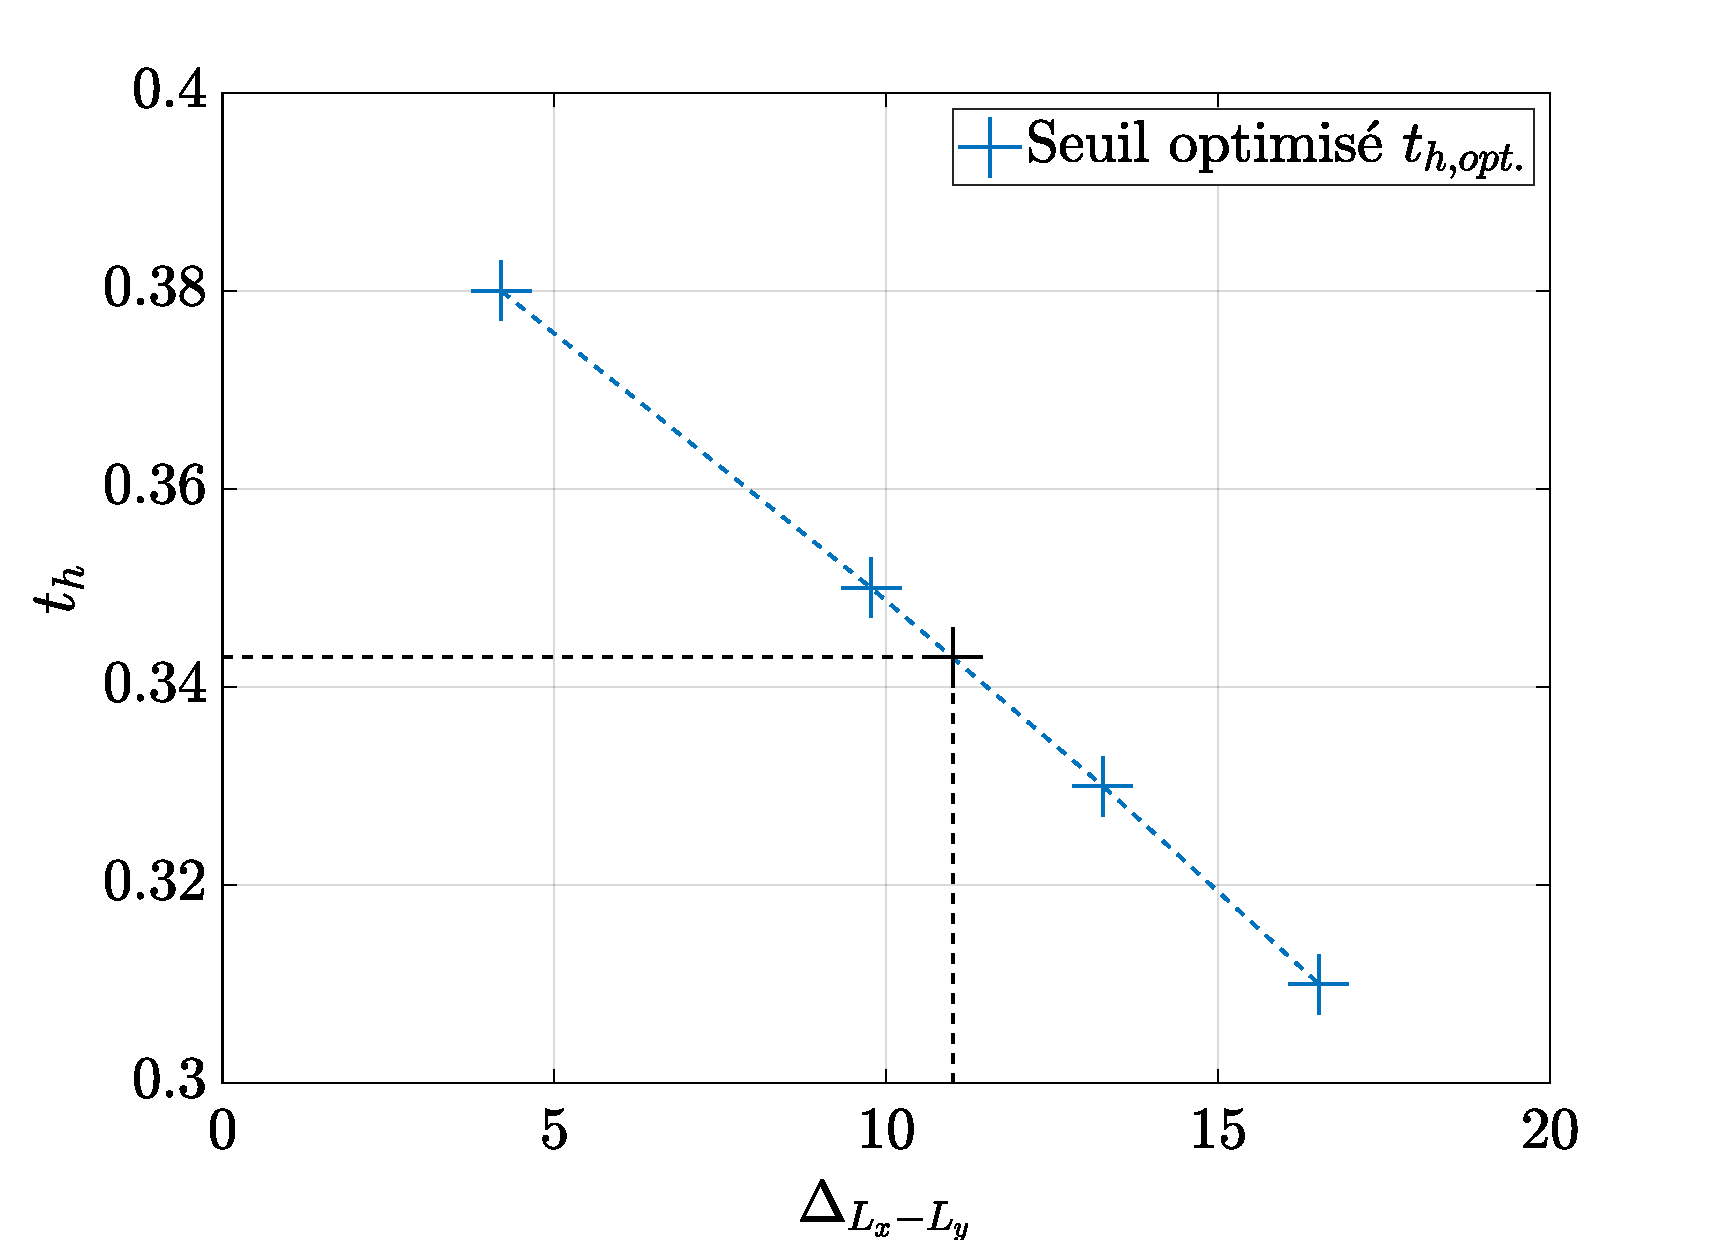
\includegraphics[width=.7\linewidth]{./figures/resultats/interpolationOpt.pdf}
\caption{Exemple d'interpolation réalisée pour une scène avec un indicateur $\Delta_{L_{1k}-L_{5k}}$ = 11 : $t_{h,interp}$ = 0,343.}
\label{fig:interpolation}
\end{figure}

\begin{table}[h]
\centering
\caption{Influence de l'indicateur d'optimisation dans l'estimation de l'erreur $MAE_{g}$.}
\label{tab:result_opt}
\begin{tabular}{L{4cm}C{2.5cm}}
\toprule
 & $\mathbf{MAE_g}$    \\
 \midrule
seuil fixe $t_h$ & 1,16 ($\pm$ 0,86)  \\
\rowcolor[HTML]{C0C0C0}
seuil optimisé $t_{h,opt}$ & 1,12 ($\pm$ 0,83) \\
\midrule
\textcolor{red}{$\mathbf{\Delta_{L_{1k}-L_{5k}}}$} & \textbf{\textcolor{red}{1,08 ($\pm$ 0,87)}}\\
\rowcolor[HTML]{C0C0C0}
$\mathbf{\Delta_{L_{2k}-L_{5k}}}$& \textbf{1,09 ($\pm$ 0,86)}\\
$\Delta_{L_{500}-L_{5k}}$ & 1,12 ($\pm$ 0,90)\\
\rowcolor[HTML]{C0C0C0}
$\Delta_{L_{1k}-L_{2k}}$ & 1,12 ($\pm$ 0,93)\\
$\Delta_{L_{500}-L_{1k}}$ & 1,12 ($\pm$ 0,95)\\
\rowcolor[HTML]{C0C0C0}
$\Delta_{L_{50}-L_{90}}$ & 1,18 ($\pm$ 0,92)\\
$\Delta_{L_{10}-L_{90}}$ & 1,29 ($\pm$ 1,09)\\
\rowcolor[HTML]{C0C0C0}
$\Delta_{L_{10}-L_{50}}$ & 1,36 ($\pm$ 1,05)\\
$\Delta_{L_{500}-L_{2k}}$ & 1,37 ($\pm$ 1,16)\\
\bottomrule
\end{tabular}
\end{table}

Les erreurs $MAE_g$ obtenues sur le corpus sont résumées dans le Tableau \ref{tab:result_opt}.
Les erreurs $MAE_g$ obtenues par interpolation avec les indicateurs $\Delta_{L_{1k}-L_{5k}}$ et $\Delta_{L_{2k}-L_{5k}}$ sont plus faibles que les approches basées sur le seuil fixe et sur les seuils optimisés. Ces deux indicateurs  sont ceux ayant les plus fortes corrélations $R$ avec l'évolution des seuils $t_{h,opt}$.
La fonction d'interpolation pour $\Delta_{L_{1k}-L_{5k}}$ est alors sur l'intervalle $\Delta_{L_{1k}-L_{5k}} \in\left[1,22;~ 15,84 \right]$: 

\begin{equation}
t_{h,interp.} = -5,70\times 10^{-3} \times \Delta_{L_{1k}-L_{5k}} +0,40.
\end{equation}

\begin{figure}[h]
\centering
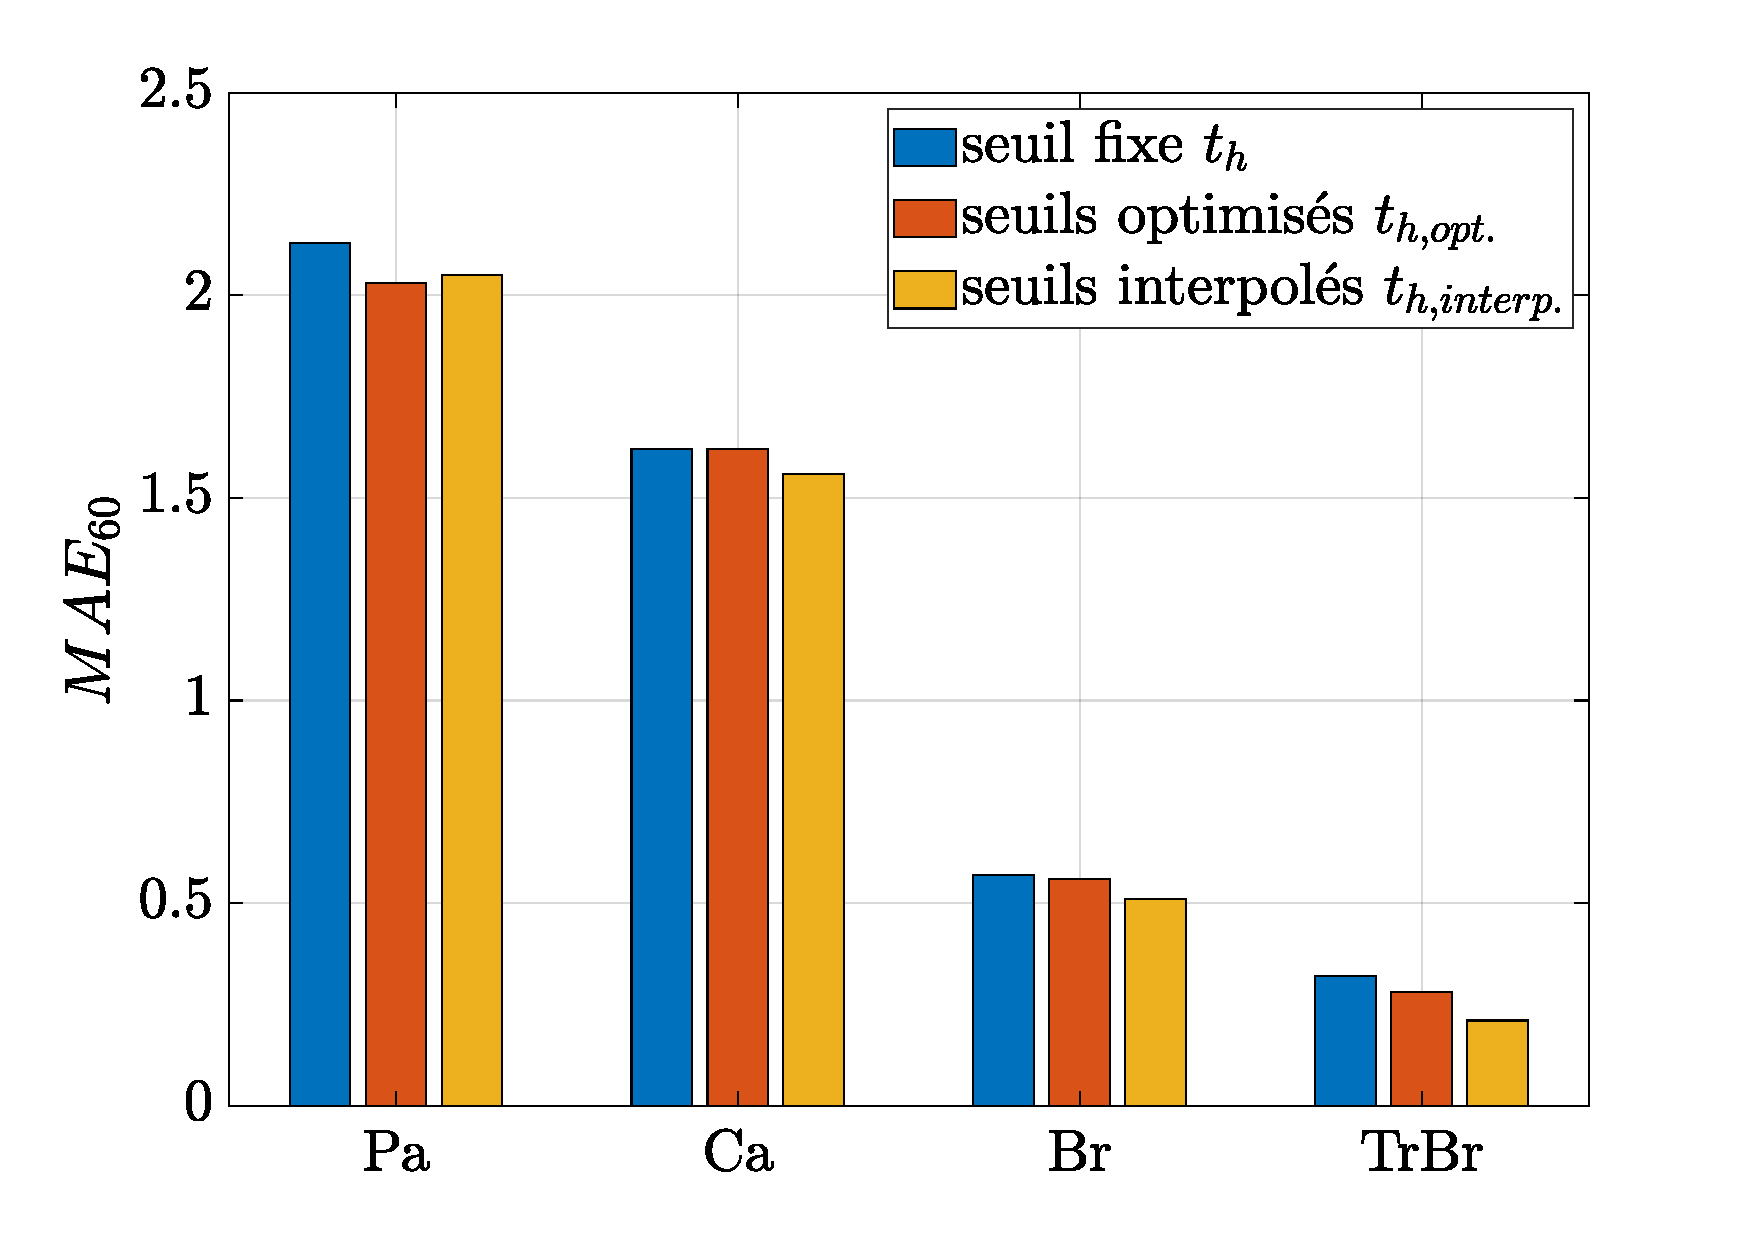
\includegraphics[width=.7\linewidth]{./figures/resultats/erreursSeuilOpt.pdf}
\caption{Influence de la méthode de seuillage (seul fixe $t_h$, optimisé $t_{h,opt.}$, interpolé $t_{h,interp.}$) à partir de l'indicateur $\Delta_{L_{1k}-L_{5k}}$ sur les erreurs $MAE_{60}$.}
\label{fig:erreurInterp}
\end{figure}

La Figure \ref{fig:erreurInterp} représente les erreurs par ambiances sonores pour la NMF IS basées sur un seuil fixe $t_h$, les seuils optimisés $t_{h,opt.}$ et sur les seuils interpolés $t_{h,interp.}$. S'il y a bien une diminution de l'erreur, celle-ci reste relativement limitée. Pour l'ambiance \textit{Parc} est le seul cas où le seuil déduit de l'interpolation génère des erreurs supérieures aux deux autres approches. Cette particularité peut être due à la sensibilité de l'erreur plus forte dans cette ambiance (voir partie \ref{part:optimisationESU} et la Figure \ref{fig:maeExpandSeuil}). Dans les autres ambiances, la déduction du seuil $t_{h,interp.}$ par interpolation réduit les erreurs. \\

Cette approche est une première piste d'ouverture pour améliorer l'estimation du niveau sonore du trafic, elle reste à être validée sur des corpus plus grands et plus variés afin d'être ajustée. 
Mais cette proposition reste intéressante en vue d'adapter la méthode aux diverses environnements sonores : par un seuil variable déduit par des indicateurs sonore de la scène, il permet de mieux prendre en compte les évolutions sur la journée ou sur l'heure des ESU auprès du capteur et donc à la NMF IS de limiter les erreurs sur l'estimation du niveau sonore du trafic.